\chapter{Testes}


\section{\textit{SmartSpace} Laico}

	O ambiente para o qual o sistema \textit{True} será projetado, desenvolvido e testado chama-se LAICO (\textbf{LA}boratório de sistemas \textbf{I}ntegrados e \textbf{CO}ncorrente), um laboratório do Departamento de Ciência da Computação da Universidade de Brasília. O LAICO possui dimensões de, aproximadamente,  $\displaystyle 7,67m$ x $\displaystyle 6,45m$ ilustrado pela Figura~\ref{fig:laico}.

	\begin{figure}[hbt]
			\begin{center}
				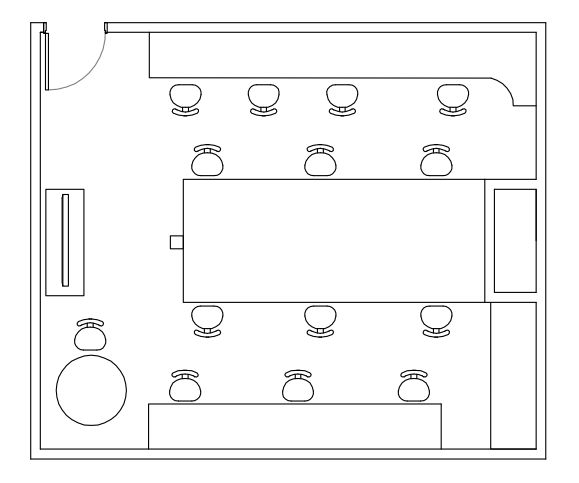
\includegraphics[scale=0.6]{figuras/4.ProblemaEProposta/laico.png}
			\end{center}
			\caption{Planta do \textit{SmartSpace} Laico.}
			\label{fig:laico}
		\end{figure}	
